\documentclass[12pt,a4paper]{article}

\usepackage[utf8x]{inputenc}
\usepackage[english]{babel}
\usepackage{xcolor}
\usepackage{hyperref}
\usepackage{parskip}
\usepackage{graphicx}
\usepackage{listings} % For code snippets
\usepackage{xcolor}
\usepackage[left=2cm, top=3cm, text={17cm, 24cm}]{geometry} 

\definecolor{codegreen}{rgb}{0,0.6,0}
\definecolor{codegray}{rgb}{0.5,0.5,0.5}
\definecolor{codepurple}{rgb}{0.58,0,0.82}
\definecolor{backcolour}{rgb}{0.95,0.95,0.92}

% Setup for code snippets
\lstdefinestyle{mystyle}{
    backgroundcolor=\color{backcolour},   
    commentstyle=\color{codegreen},
    keywordstyle=\color{magenta},
    numberstyle=\tiny\color{codegray},
    stringstyle=\color{codepurple},
    basicstyle=\ttfamily\footnotesize,
    breakatwhitespace=false,         
    breaklines=true,                 
    captionpos=b,                    
    keepspaces=true,                 
    numbers=left,                    
    numbersep=5pt,                  
    showspaces=false,                
    showstringspaces=false,
    showtabs=false,                  
    tabsize=4
}

% Path to images
\graphicspath{ {./images/} } 

% Setup for hyperrefs
\hypersetup{
    colorlinks=true,
    linkcolor=blue,
    filecolor=magenta,      
    urlcolor=blue,
}

% TODO command
\newcommand{\todo}[1]{\textcolor{red}{\textbf{[[TODO]]}} $\Rightarrow$ \textbf{#1}}
% Globally disable indentation -> package parskip
\setlength{\parindent}{0pt}

\begin{document}
    \begin{titlepage}
        \begin{center}
            \vspace*{1cm}
    
            \Large{\textbf{Project IIS}}
    
            \vspace{0.5cm}
            Monitoring of SSL connection
                
            \vspace{1.5cm}
            
            \textbf{Pavel Yadlouski (xyadlo00)}
    
            \vfill
                
            \vspace{0.8cm}
        
            Brno University of Technologies\\
            September, 2020
                
        \end{center}
    \end{titlepage}
    
    \tableofcontents
    \newpage

    \section{Introduction}
    Aim of this project is to create simple CLI application, that can monitor SSL communication.
    Here monitoring means to aggregate input file \textbf{and / or} given network interface.  
        

    \section{Architecture}
    \begin{center}
        \begin{figure}[h!]
            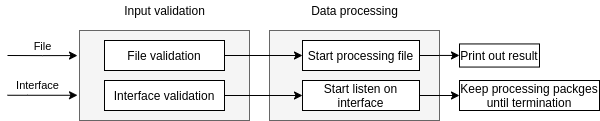
\includegraphics[scale=0.7]{sslsniff.png}
        \end{figure}
    \end{center}
    Whole program contains two main parts:
    \begin{enumerate}
        \item input validation
        \begin{enumerate}
            \item check if file exists and with supported extension
            \item check if given interface exists and can be opened for listening
        \end{enumerate}
        \item data processing
        \begin{enumerate}
            \item aggregate given file
            \item start live aggregation of incoming traffic on given interface
        \end{enumerate}
    \end{enumerate}
    The result of file aggregation is written to the standard output as soon as
    aggregation is completed. 
    If interface is set, then program start listening on given interface and aggregate 
    incoming packets. When the last packet of any connection is aggregated, 
    then it the result of the aggregation for this particular connection would be 
    written to the standard output. 

    \subsection{Storing connections}
    As data structure for storing connections information doubly linked list is used.
    This data structure was chosen was chosen for its simplicity of implementation 
    and use. Also, despite of hash table, doubly linked list very flexible from
    the memory usage point of view: doubly linked list doesn't have fix size, so
    can grow as much as it would be necessary. In case of resizing hash table 
    require recalculating hashes for every item, but doubly linked list doesn't
    have this problem. There just insert to the any side of the list. Also as 
    each element of list has pointer to previous and next elements, then deleting
    of element is quite trivial: reset pointers between siblings of given connection
    and delete it.

    The biggest disadvantage of doubly linked list is high searching complexity.
    For every package whole list can be looked through. But in this application 
    it is not significant, because is very simple. 

    \subsection{Packet processing}

    When program is started and first packet is came, then it would be set as 
    the first element in the list. After that for every packet would be found 
    corresponding entry in list (based on comparing source and destination 
    IP addresses and ports). If entry doesn't exist, then this packet would be
    inserted to the beginning of the list with setting up links for next 
    and previous entries.
    
    When processing file, any packet wouldn't be deleted from list during 
    process. Because we don't know if later in the file there is no more 
    packets that corresponds to this particular entry. But during aggregation 
    of interface every finished connection (based on TCP flags) is freed from 
    the list.


    \subsection{Multithreading}
    Program use separated threads for processing file and interface 
    simultaneously. Main thread would wait first on file processing thread 
    and then on the interface thread.

    
    \section{Implementation}
    Program contains two parts: checking of input parameters and package aggregation by itself.
    First part presents in file \textit{sslsniff.c}. Also setup functions for aggregation are 
    called there. Second part is represented in file \textit{functions.c} with header 
    \textit{functions.h}. 

    \subsection{Data structures}
    There are several auxiliary data structures for packet aggregation. 

    \subsection{TLS extensions}
    For processing SSL/TLS extensions there is following structure
    \lstset{style=mystyle}
    \begin{lstlisting}[language=C]
 typedef struct {
     char ext_type_hex[5];
     unsigned int ext_type;
     char ext_len_hex[5];
     unsigned int ext_len;
     char *data;
 } extention;
    \end{lstlisting}
    
    This structure helps to go through extensions in SSL/TLS headers and find extension with SNI.
    To check type of extension there are two element \textit{ext\_type\_hex} and \textit{ext\_type}.
    First represents hexadecimal value of type and after conversion decimal value is stored in 
    second element. Same idea is used for getting length of extension data. First extract hexadecimal
    from corresponding position and store to array, then convert this array with hexadecimal values 
    to decimal number. This solution is used because type and length of extension is stored on 2 bytes
    both, so there is need to convert this to 2 bytes to one decimal value.

    So, for getting SNI name there is loop through all extensions. In this loop there is \textit{if}
    statement which checks type of extension and if it is equal to 0, then this extension would contain
    SNI name in its data. In the end, if this type of extension presents, SNI is extracted and stored 
    to corresponding element in TLS connection structure.
    
    \subsection{TLS connection}
    Each SSL/TLS connection is represented by following structure
    \begin{lstlisting}[language=C]
 typedef struct tls_conn{
     u_int src_ip, dst_ip;
     u_int16_t src_port, dst_port;
     struct timeval timestamp;
     double duration;
     char *sni;
     u_int packet_count;
     u_int bytes;
     u_int addr_size;
     bool server_fin, server_ack, client_ack, client_fin;
     bool last_ack;
     struct tls_conn *prev, *next;
 } tls_connection;
    \end{lstlisting}

    There are source and destination IP addresses in integer format. The reason for storing addresses 
    in integer format is that comparing of integers is faster that comparing of strings. Conversion 
    to human ridable format is made only when result of aggregation should be written to standard 
    output. Also for detecting that packet is corresponds to given connection there are source and
    destination ports. 

    For aggregation purpose there are elements for storing amount of packets in given connection,
    duration and bytes. Durations of connections is founded as result of subtraction \textit{timestamp} 
    (represents timestamp of first packet aggregated in given connection) and timestamp of new packet
    for corresponding connection. For subsection of timestamps there is function \textit{time\_diff} 

    For interface aggregation end of the communication is detected based on flags 
    \textit{server\_fin, server\_ack, client\_ack, client\_fin, last\_ack}. This flags corresponds 
    to TCP flags of given connection. Connection is considered closed when flag \textit{last\_ack} 
    is set to \textit{True}. This happens when all of flags \textit{server\_fin, server\_ack, 
    client\_ack, client\_fin} also have value \textit{True}. 

    As doubly linked list is used, then there are also pointers to next element (connection) and 
    previous. 

    On step of input validation \textit{cleanup} function is set to be triggered on signal 
    \textit{SIGINT}. This step is necessary for interface aggregation. Processing of live connection 
    is not limited, so this setup insures that data will be freed of interruption.

    \section{Problems and limitations}
    \subsection{CPU usage}
    There is problem where in 1 from 10 runnings after random amount of packets program would 
    load one core up to 100\% and stop writing logs to standard output. Reason of this wight be 
    some infinite loop in code, but this problem isn't solved.  

    \subsection{Performance}
    As for storing data during aggregation doubly linked list is used, with big amount of 
    live connection or on long runs performance of application is going down due to searching
    time in data structure.

    \newpage
    \nocite{*}
    \bibliographystyle{style}
    \bibliography{sample}


\end{document}